\documentclass{article}
\usepackage[margin=2cm]{geometry}

\input{./basic-tex-config/preamble.tex}

\graphicspath{{./images/}}

\title{ЛАБОЛАТОРНАЯ РАБОТА ПО КУРСУ\\ <<КВАНТОВЫЙ КОМПЬЮТЕР>>\\
Двухкубитовые квантовые схемы}
\date{Санкт-Петербург, 2017}
\author{Плотников Антон, А4101}

\begin{document}

\maketitle
\newpage

\section{Цель работы}

Изучение простейших двухкубитовых квантовых логических схем.

\section{Задачи}

\begin{enumerate}
  \item Изучение работы квантовых логических схем, составленных из
    элементов алгоритмов CNOT, X, Z и H.

  \item Прогнозирование результатов виртуального эксперимента и сравнение
    результатов теоретических и экспериментальных расчетов.
\end{enumerate}

\section{Методика проведения исследования}

Собираем квантовую схему используя квантовые логические элементы CNOT, X, H и
Z, подаем на вход цепочки элементов двухкубитовое состояние кубит, получаем
выходное двухкубитовое состояниие и, используя матричное представление схемы,
сравниваем результаты теоретических расчетов с полученными экспериментальными
данными.

\section{Анализ погрешностей}

Пусть $\ket{\phi1}$ – состояние, соответствующее первой альтернативе, а
$\ket{\phi2}$ – состояние, соответствующее второй альтернативе. Пусть перед
измерением система находилась в состоянии $c_1\ket{\phi1} + c_2\ket{\phi2}$.
Тогда с вероятностью $|c_1|^2$ измерение даст первый результат, и система
окажется после измерения в состоянии $\ket{\phi1}$, а с вероятностью $|c_2|^2$
измерение даст второй результат, и система окажется после измерения в состоянии
$\ket{\phi2}$.

\section{Результаты}

Исходный вектор: 
 
\begin{align}
  \ket{\phi_1} &= \ket{1}
  \\
  \ket{\phi_2} &= \ket{1}
  \\
  \ket{\phi} &= \ket{\phi_1} \otimes \ket{\phi_2} =\begin{pmatrix} 0 \\ 1
  \end{pmatrix} \otimes \begin{pmatrix}  0 \\ 1 \end{pmatrix}= \begin{pmatrix}
  0 \\ 0 \\ 0 \\ 1 \end{pmatrix}
\end{align}

Квантовая схема:
\begin{figure}[H]
  \center{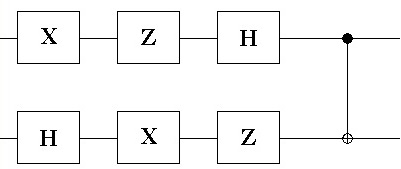
\includegraphics[width=0.5\textwidth]{Sx-ma}}
\end{figure}

Теоретические расчеты:
 
\begin{align}
  U_1 &= HZX=\frac{1}{\sqrt{2}}\begin{pmatrix}\begin{array}{rr} 1 & 1 \\ 1 & -1
  \end{array} \end{pmatrix}\begin{pmatrix} \begin{array}{rr}1 & 0 \\ 0 & -1
  \end{array}\end{pmatrix}\begin{pmatrix} 0 & 1 \\ 1 & 0
  \end{pmatrix}=\frac{1}{\sqrt{2}}
  \begin{pmatrix}\begin{array}{rr} -1 & 1 \\ 1 & 1 \end{array}\end{pmatrix}
  \\
  U_2 &= ZXH = \begin{pmatrix}\begin{array}{rr} 1 & 0 \\ 0 & -1
  \end{array}\end{pmatrix}\begin{pmatrix} 0 & 1 \\ 1 & 0
  \end{pmatrix}\frac{1}{\sqrt{2}} \begin{pmatrix}\begin{array}{rr} 1 & 1 \\ 1 &
  -1 \end{array} \end{pmatrix} = \frac{1}{\sqrt{2}}
  \begin{pmatrix}\begin{array}{rr} 1 & -1 \\ -1 & -1 \end{array}\end{pmatrix}
  \\
  U &= U_1 \otimes U_2 = \frac{1}{\sqrt{2}} \begin{pmatrix}\begin{array}{rr} -1 &
  1 \\ 1 & 1 \end{array} \end{pmatrix} \otimes \frac{1}{\sqrt{2}}
  \begin{pmatrix}\begin{array}{rr} 1 & -1 \\ -1 & -1 \end{array} \end{pmatrix} =
  \frac{1}{2} \begin{pmatrix}\begin{array}{rrrr} -1 & 1 & 1 & -1 \\ 1 & 1 & -1 &
  -1 \\ 1 & -1 & 1 & -1 \\ -1 & -1 & -1 & -1 \\ \end{array}\end{pmatrix}
  \\
  CNOTU\ket{\phi} &= \begin{pmatrix} 1 & 0 & 0 & 0 \\ 0 & 1 & 0 & 0 \\ 0 & 0 &
  0 & 1 \\ 0 & 0 & 1 & 0 \end{pmatrix}\frac{1}{2}
\begin{pmatrix}\begin{array}{rrrr} -1 & 1 & 1 & -1 \\ 1 & 1 & -1 & -1 \\ 1 & -1
                                      & 1 & -1 \\ -1 & -1 & -1 & -1
\end{array}\end{pmatrix} \begin{pmatrix} 0 \\ 0 \\ 0 \\ 1 \end{pmatrix} =
\frac{1}{2} \begin{pmatrix}\begin{array}{r} -1 \\ -1 \\ -1 \\ -1
\end{array}\end{pmatrix}
\end{align}

Экспериментальные расчеты:

\begin{figure}[H]
  \center{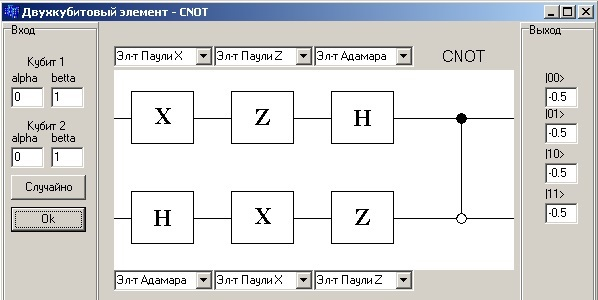
\includegraphics[width=0.85\textwidth]{3_Sx}}
\end{figure}

\textbf{\large 5. Выводы}

Изучив работу квантовых логических схем, составленных из элементов алгоритмов
CNOT, X, Z и H, сравнили результаты теоретических и экспериментальных расчетов.
В результате получили одинаковые результаты.

\end{document} 
